\usetikzlibrary{arrows, calc, shapes.geometric}

\tikzstyle{new} = [
    rectangle, 
    rounded corners, 
    minimum width=3cm, 
    minimum height=1cm,
    text centered, 
    text width=3cm,
    draw=black, 
    fill=red!30
]
\tikzstyle{old} = [
    rectangle, 
    rounded corners, 
    minimum width=3cm, 
    minimum height=1cm,
    text centered, 
    text width=3cm,
    draw=black, 
    fill=blue!30
]
\tikzstyle{arrow} = [thick,<->,>=stealth]

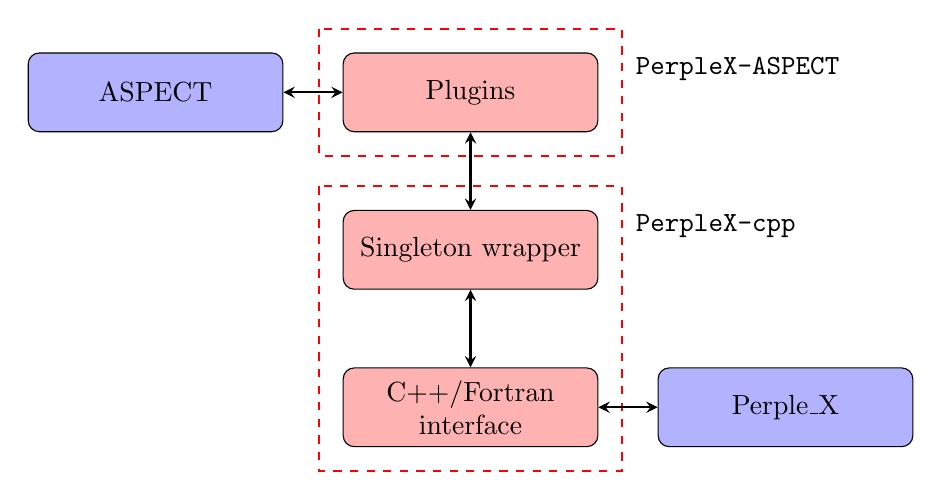
\begin{tikzpicture}[node distance=2cm]
    \node (aspect) [old] {ASPECT};
    \node (plugins) [new, right of=aspect, xshift=2cm] {Plugins};
    \node (singleton) [new, below of=plugins] {Singleton wrapper};
    \node (interface) [new, below of=singleton] {C++/Fortran interface};
    \node (perplex) [old, right of=interface, xshift=2cm] {Perple\_X};
    
    \draw[red, thick, dashed, label=test] 
        ($(plugins.north west)+(-0.3,0.3)$) rectangle 
        ($(plugins.south east)+(0.3,-0.3)$);
    \draw[red, thick, dashed]     
        ($(singleton.north west)+(-0.3,0.3)$) rectangle 
        ($(interface.south east)+(0.3,-0.3)$);
        
    \node (label1) [
        right of=plugins,
        xshift=1.6cm, 
        yshift=0.3cm,
        text width=3cm
    ] {\texttt{PerpleX-ASPECT}};
    \node (label2) [
        right of=singleton, 
        xshift=1.6cm, 
        yshift=0.3cm,
        text width=3cm
    ] {\texttt{PerpleX-cpp}};
    
    \draw [arrow] (aspect) -- (plugins);
    \draw [arrow] (plugins) -- (singleton);
    \draw [arrow] (singleton) -- (interface);
    \draw [arrow] (interface) -- (perplex);
\end{tikzpicture}